\documentclass[a4paper, fontsize=10pt]{scrartcl}
\usepackage[utf8]{inputenc}
\usepackage[ngerman]{babel}
\usepackage{stmaryrd}
\usepackage{amsfonts}
\usepackage{amsmath}
\usepackage{mathpazo} %schickere Schriftart für Text
\usepackage{MnSymbol} %schickere Symbole
\usepackage{graphicx}
\usepackage{amsthm}
\usepackage{shadethm}
\usepackage[all,2cell,ps]{xy}
\usepackage{setspace}

\usepackage{listings}
\usepackage{hyperref} %Hyperlinks einfügbarisieren
\usepackage{fancyvrb} %verbatim mit mehr Variationen
\usepackage{listings} %Quellcode mit listings einbinden
\usepackage{moreverb}
\usepackage{tocloft} %tableofcontent mit Optionen
\usepackage{tikz}
\usetikzlibrary{shapes}
\usepackage{algorithm}
\usepackage{algorithmic}
\usepackage{multicol}
\usepackage{soul}
\usepackage[makeroom]{cancel}


\definecolor{lightgray}{gray}{0.9}

\usetikzlibrary{arrows}
% \usepackage{ulem} %neue Befehle für Unterstriche
\usetikzlibrary{arrows,calc,shapes.multipart,chains}
\usetikzlibrary{calc,positioning}

\renewcommand{\algorithmicrequire}{\textbf{Input:}}
\renewcommand{\algorithmicensure}{\textbf{Output:}}

\lstloadlanguages{Java} %Standardmäßig Java vorher laden
% Standard-Layout für die Code-Umgebung (alle Sprachen)
\lstset{%
      basicstyle=\small\ttfamily,
     showspaces=false,
     showtabs=false,
     columns=fixed,
     numbers=left,
     frame=none,
     numberstyle=\tiny,
     breaklines=true,
     showstringspaces=false,
     xleftmargin=1cm,
     tabsize=4
}%
\setlength\topmargin{-1cm}
\textheight 23cm
\textwidth 14cm
\setlength\oddsidemargin{1cm}
\setlength\evensidemargin{3.5cm}
\parindent=0pt
\setlength{\saveparindent}{\parindent}
%\pagestyle{empty}
\newcommand{\rem}[1]{} %rem-Kommentiermöglichkeit
\definecolor{dg}{rgb}{0.8,0.8,0.8}		%definiert dunkelgrau
\definecolor{hg}{rgb}{0.95,0.95,0.95}	%definiert hellgrau
%%%%%%%%%%%%%%%%%%%%%%%%%%%%%%%%%%%%%%%%%%%%%%%%%%%%%%%%%%%%%%%%%%%%%%%%%%%%%%%%%%%  
 
\begin{document} 

{\huge{Algorithmendesign} \hfill \large{ Gruppe 2}}\\  
{\large Lösungen zu Übungsblatt 10} \hfill Max Bannach\\
{\large WS 13/14}
\begin{flushright}Markus Richter (614027)\end{flushright}
\rule{\textwidth}{.3mm}

\section*{Aufgabe 10.1 Online-Interval-Scheduling}
\subsection*{Teilaufgabe 1)}

Nicht stark $\rho$-kompetitiv bedeutet\smallskip

  \begin{center}
    $\forall \cal{A}$ $\forall \rho$ $\exists X: \cal{A}(\textrm{X}) <$ $\dfrac{\textsc{OPT(X)}}{\rho}$
  \end{center}
\smallskip

Das lässt sich relativ einfach anhand einer Strategie für einen Gegenspieler zeigen. Siehe hierfür auch das Tantau Skript Seite 36. Dem Online-Algorithmus wird im Grunde ein Intervall nach dem anderen vorgesetzt und dieser entscheidet, ob er es schedult oder nicht. Der Gegenspieler
\begin{enumerate}
  \item produziert die Intervalle $[1,2], [2,3), [3,4)$ usw. bis der Algorithmus sich das erste Mal bei einem Intervall für \emph{schedule} entscheidet. 
  \item Nun produziert er Intervalle der Größe $\frac{1}{\rho+1}$ und positioniert sie alle innerhalb des Intervalls, für welches sich der Algorithmus vorher entschieden hat.
\end{enumerate}

Der Gegenspieler produziert auf diese Weise mindestens $\rho+2$ Intervalle. Der Algorithmus entscheidet sich also nur für ein Intervall, obwohl $\rho+1$ Intervalle möglich wären. Damit ist die kompetitive Rate schlechter als $\rho$. \begin{flushright}$\blacksquare$\end{flushright} \bigskip

Gegeben sei folgendes Beispiel:

  \begin{center}
    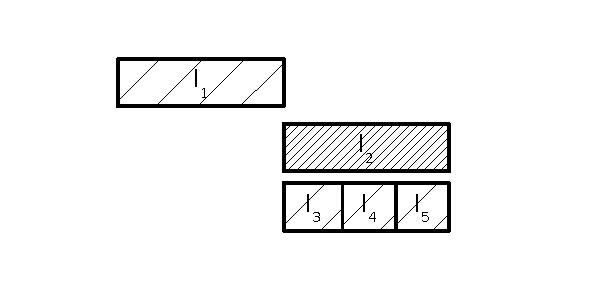
\includegraphics[scale=0.7]{aufgabe1a.pdf}
  \end{center}
  
Sei $\rho=2$. Entscheidet sich der Algorithmus für $I_2$, so platziert der Gegenspieler $I_3$ bis $I_5$ unterhalb von $I_2$. Damit gilt:
$1<\dfrac{4}{2}$


\subsection*{Teilaufgabe 2)}

Um zu zeigen, dass auch für die Summe der Ausführungszeiten eines Schedules für kein festes $\rho \in \mathbb{N}$ einen stark $\rho$-kompetitiven Algorithmus gibt, verfährt man analog zu oben und entwirft eine Gegenspieler-Strategie:
\begin{enumerate}
  \item Der Gegenspieler generiert ein Intervall nach dem anderen mit gleicher Länge mit Hilfe von $f_i$ und $s_i$.
  \item Entscheidet sich der Algorithmus das erste mal für ein Intervall $I_j$, so produziert der Gegenspieler ein Intervall der Länge $(\rho +1)(f_j-s_j)$ und platziert ihn so, dass der Algorithmus ihn nicht mehr schedulen kann. Erst nach Ende dieses Intervalls produziert der Gegenspieler wieder gleich lange Intervalle. 
\end{enumerate}\smallskip

Es gilt also:\smallskip
  \begin{center}
  $ \dfrac{ \cal{A}\textrm{(X)}}{\textsc{OPT}(X)}\geq \dfrac{\sum\nolimits_{x_i\in S}|f_i-s_i|}{\sum\nolimits_{x_i\in S}(\rho+1)|f_i-s_i|}  \Leftrightarrow  \dfrac{\cal{A}\textrm{(X)}}{\textsc{OPT}(X)} \geq \dfrac{1}{\rho +1 }$

  \end{center}
\smallskip

Gelten muss jedoch
  \begin{center}
 $ \dfrac{ \cal{A}\textrm{(X)}}{\textsc{OPT}(X)}\geq \dfrac{1}{\rho }$
  \end{center}



Daraus folgt, dass die kompetitive Rate schlechter ist als $\rho$. \begin{flushright}$\blacksquare$\end{flushright}


  \begin{center}
    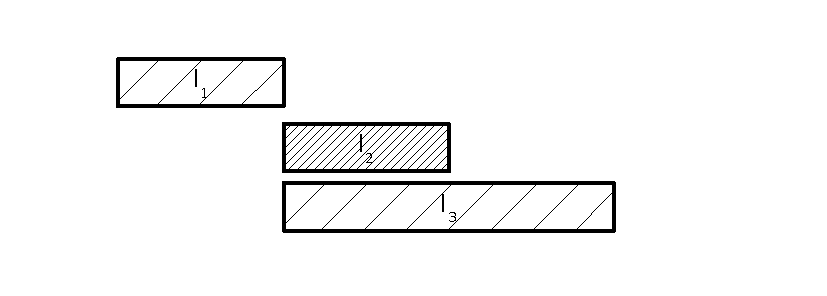
\includegraphics[scale=0.7]{aufgabe1b.pdf}
  \end{center}
  
\newpage

\section*{Aufgabe 10.2 Feuerwehr}

\subsection*{Teilaufgabe 1}

Im Folgenden nehme ich an, dass die Linienmenschen einen begrenzten Bereich der unendlich langen Straße (wie soll das gehen?) bebaut haben, andernfalls hätten sie nicht wenig natürliche Resourcen. Mit wenig natürlichen Resourcen können sie auch nur endlich viele Wagen bauen und damit nur einen endlich langen Bereich der Straße abdecken.\smallskip

Angenommen der Algorithmus iteriert von einem Schritt oder Zeitpunkt zum nächsten. Zu jedem solchen Zeitpunkt $i$ bricht \emph{ein} Brand aus. Dann beschreibt $X=x_1,x_2,\dots,x_n$ mit $x_i\in [A,E]$ eine Stelle im Linienland, an der zum Zeitpunkt $i$ ein Brand ausbricht. $A$ und $E$ beschreiben die Grenzen, $A$ ist der Anfang und $E$ das Ende.\smallskip

$Y=y_1,y_2,\dots,y_n$ mit $y_i\in \{1,\dots,k\}$ ist dann die Aktion zum Zeitpunkt $i$. Die Aktion besagt welcher der $k$ Wagen den Brand löschen soll. Damit die Wagen $w$ wissen, wohin sie fahren müssen, müssen sie wissen wo sie sich zum Zeitpunkt $i$ befinden. Sei dies ihre Position $p_{w_{i}}$. \smallskip

Das Optimierungsproblem $\Pi$ besteht also nun darin die Entfernungen $p_{w_{i-1}}$ und $p_{w_{i}}$ aller Wagen $w$ zwischen zwei aufeinander folgenden Zeitpunkten $i-1$ und $i$ zu minimieren. 

\subsection*{Teilaufgabe 2}
Die Idee ist nun den bebauten Bereich der Straße in gleichlange Partitionen aufzuteilen. Für die Länge einer Partition gilt $l=\frac{E}{k}$. Jeder Wagen hat also seine Partition. Zu Beginn wird jeder Wagen in der Mitte seiner Partition positioniert. Initial müssen alle Wagen an ihre Position gebracht werden, was in einer Wegstrecke $\frac{k}{2}\cdot E$ resultiert.\smallskip

Damit man weiß welcher Wagen für einen Brand $x_i$ zuständig ist, wird die zuständige Partition wie folgt ermittelt:
$(x_i\mod l)+1$.\smallskip

Im schlimmsten Fall kann es passieren, dass ein Feuer immer an den Grenzen einer Partition ausbricht, z. B. bei $0$ und $l$, sodass ein Wagen ständig hin und her fahren muss. Ein Offline-Algorithmus weiß das bereits im Vorfeld und kann gleich zu Beginn die Wagen direkt an die Grenzen stellen, sodass es nur initial einer Bewegung bedarf und danach keiner weiteren.\smallskip

Für die kompetitive Rate -- wobei $n$ für die Anzahl der Zeitpunkte steht -- bedeutet das\smallskip

\begin{center}
  $\textsc{CR}(\cal{A}(\textrm{X}))=$$\dfrac{\frac{k^2}{2}\cdot l+l\cdot n}{l + 0}=\dfrac{k^2}{2}+n$
\end{center}

Man sieht also, dass der Ausdruck beliebig wächst für $n$, außerdem gilt $k^2>k$. Daraus resultiert, dass der Algorithmus nicht k-kompetitiv ist. 

\newpage

\section*{Aufgabe 10.3 Flucht der Kuh}

\subsection*{Teilaufgabe 1}

Die denkbar schlechteste Position für das Verhältnis ist die, bei der die Kuh das Loch knapp verfehlt, dann eine möglichst lange Strecke in die entgegengesetzte Richtig hin und zurück laufen muss, zuzüglich die direkte Entfernung Ausgangspunkt zum Loch. Man will also den Ausdruck\smallskip
$\dfrac{ \cal{A}\textrm{(X)}}{\textsc{OPT}(X)}$ maximieren, indem man den Zähler möglichst maximiert und den Nenner minimiert.\bigskip

Sie das Loch an Position $-10$. Die Kuh läuft dann eine Strecke von 90 Metern, bis sie das Loch gefunden hat. Die Offline-Version des Algorithmus bräuchte aber nur $10$ Meter, was der optimalen Strecke entspricht. Das Verhältnis in diesem Beispiel ist also $\dfrac{90}{10}=9$.

\begin{center}
    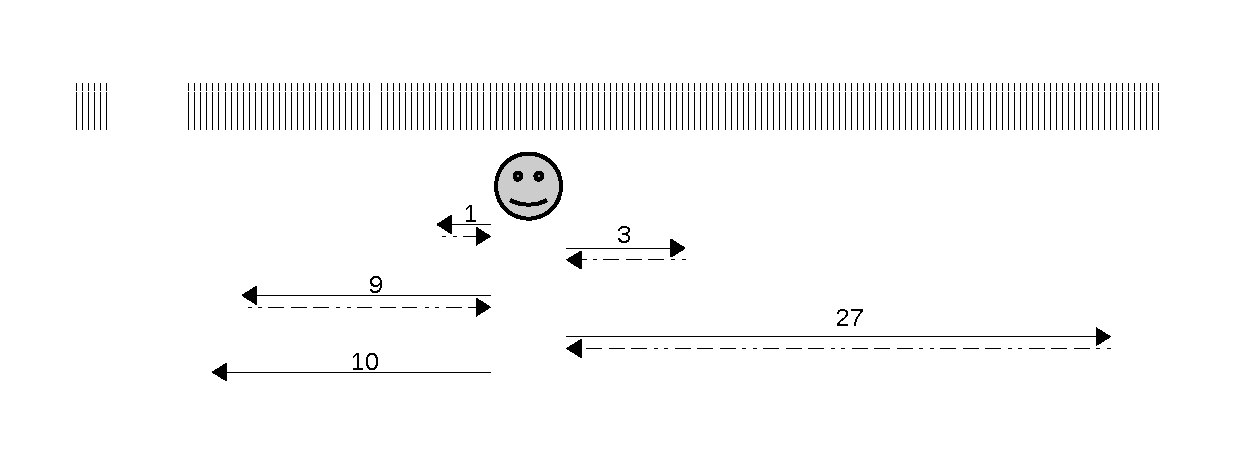
\includegraphics[scale=0.7]{aufgabe2a.pdf}
  \end{center}
  

\subsection*{Teilaufgabe 2}

Für den schlimmsten Fall, also einem Loch bei $3^k+1$, wobei $k$ der Anzahl der Richtungswechsel entspricht, beträgt die optimale Strecke eben $3^k+1$. Der Algorithmus jedoch läuft\\
$2\cdot\sum\nolimits_{i=0}^{k+1}3^i+(3^k+1)=3^{k+2}-1+(3^k+1)=3^{k+2}+3^{k}<10\cdot (3^k+1)<10\cdot OPT$\smallskip

Daraus folgt, dass die Strategie der Kuh maximal das 10-fache des optimalen Weges zurücklegt.

\subsection*{Teilaufgabe 3}

Ja, indem man verdoppelt statt zu verdreifachen. Dann ist der Worst-Case nämlich $2^k+1$. Daraus ergibt sich für den Algorithmus:\smallskip

$2\cdot \sum\nolimits_{i=0}^{k+1}2^i+(2^k+1)=2\cdot(2^{k+2}-1)+(2^k+1)<8\cdot 2^k+2^k<9\cdot OPT$\smallskip


Die kompetitive Rate sinkt dann also von 10 auf 9.
\end{document}
